%\vspace{-0.1in}
\section{Introduction}
\label{sec:intro}

In big-data compute clusters, jobs arrive online and compete to share the
cluster resources. In order to best utilize the cluster and to ensure
that jobs also meet their service level objectives, efficient
scheduling is essential. However, as jobs arrive online, their runtime
characteristics are not known a priori. Due to this lack of
information, it is challenging for the cluster scheduler to determine
the right job execution order that optimizes scheduling metrics
such as maximal resource utilization or application service level objectives.

An effective way to tackle the challenges of cluster scheduling is to
learn the runtime characteristics of pending jobs, as accurately
estimating job runtime characteristics allows the scheduler to
exploit offline scheduling algorithms that are known to be optimal,
\eg Shortest Job First for minimizing the average completion time.
%
Indeed, there have been a large amount of work \cite{tetrisched,
  morpheus, 3Sigma, IfYouAreLateDontBlameUs:socc14,
  DontCryOverSpilledRecords, corral, perforator:socc2016, cdef:atc18} on learning
job runtime characteristics to facilitate cluster job
scheduling.
%        , \eg to leverage optimal offline algorithms using the estimated job runtime information.
% or improve avaialbility by predicting error rates~\cite{cdef:atc18}}.
% error rates of what?
%{Indeed, there have been a large amount of work on
%learning job runtime characteristics online to facilitate cluster job
%scheduling, \eg to leverage optimal offline algorithms to minimize job
%compeltion time \cite{tetrisched, morpheus, 3Sigma,
%IfYouAreLateDontBlameUs:socc14, DontCryOverSpilledRecords} or better resource
%utilization \cite{shufflewatcher, corral}, or meeting deadlines \cite{morpheus,
%3Sigma} or improving availability by predicting error rates \cite{cdef:atc18}
%or optimize dollar cost in virtual machine scheduling
%\cite{perforator:socc2016, stratus:socc2018}.}

In essence, all of the previous learning algorithms learn job
runtime characteristics from observing historical executions of the
same jobs, which execute the same code but process different sets of
data, or similar jobs, which have matching features such as the same
application name, the same job name, or the same user who executed the
job.

The effectiveness of the above {\em history-based} learning schemes
critically rely on two conditions to hold true: 
(1) The jobs are recurring; (2) The performance of the same or
similar jobs will remain consistent over time.

In practice, however, the two conditions often do not hold true.
First, many previous work have acknowledged that not all jobs are
recurrent. For example, in the traces used in Corral \cite{corral} and
Jockey~\cite{jockey:eurosys2012}, only
40\% of the jobs are recurrent, and Morpheus \cite{morpheus} shows that
only 60\% jobs are recurrent.
%
Second, even the authors of history-based prediction schemes such as
3Sigma~\cite{3Sigma} and Morpheus~\cite{morpheus} strongly argued why
runtime properties of jobs, even with the same input, will not remain
consistent and will keep evolving. The primary reason is that updates
in cluster hardware, application software, and user scripts to execute
the cluster jobs can affect job runtime characteristics.
%
%\commentaj{Why \S\ref{sec:back} mentioned below?}
Third, our own analysis of two production cluster traces (\S\ref{sec:accuracy}) have also shown that historical job runtime
characteristics have considerable variations.

In this paper, we explore an alternative approach to learning runtime
properties of distributed jobs online to facilitate cluster
job scheduling.
%
The approach is motivated by the following key observations about
distributed jobs running on shared clusters: (1) a job typically has a
{\em spatial dimension}, \ie it typically consists of many tasks; and (2)
the tasks (in the same phase) of a job typically execute the same code
and process different chunks of similarly sized
data~\cite{googleClusterData2011-2Schema,
  personalCommunication:MarkAstley}.  These observations suggest that
if the scheduler first schedules a few sampled tasks of a job, known as
pilot tasks, to run till finish, it can use the observed runtime
properties of those tasks to accurately estimate those of the whole
job.  Effectively, such a {\em task-sampling-based} approach learns job
properties in the spatial dimension.  We denote the new learning
scheme as \slearn.

Intuitively, by using the execution of pilot tasks to predict the
properties of other tasks, \lTechnique avoids the primary drawback of
history-based learning techniques, \ie relying on jobs to be recurring
and job properties to remain stationary over time.  However, learning
in space introduces two new challenges: (1) its estimation accuracy
can be affected by the variations of task runtime properties, \ie task skew; 
(2) delaying scheduling the remaining tasks of a job till the
completion of sampled tasks may potentially hurt the job's completion
time.

In this paper, we perform a comprehensive comparative study
of history-based learning (learning in time) and sampling-based learning
(learning in space), to systemically answer the following questions:
\begin{enumerate}
\item Can learning in space be more accurate than learning in time?
\item Can {delaying scheduling} the remaining tasks of a job till the completion
of sampled tasks be more than compensated by the improved accuracy, so
that the overall job performance, \eg completion time, is improved?
\end{enumerate}

We answer the first question via quantitative analysis, and trace and
experimental analysis based on two production job traces, a public
cluster trace from Google~\cite{googleTraceGithub} and a private trace
from 2Sigma~\cite{2Sigma:website}.  We answer the second
question by designing a generic scheduler that schedules jobs based on
job runtime estimates to optimize a given performance metric, \eg
average job completion time (JCT), and then plug into the scheduler
different prediction schemes, in particular, learning in time and
learning in space, to compare their effectiveness
using three production job traces.

\if 0
  Second, scheduling pilot tasks first may elongate the JCT of the newly
arriving job itself whose other tasks cannot start until the pilot
tasks finish. This is again typically insignificant for following reason:
job scheduling is of high relevance in a busy
cluster (when there is a backlog of jobs in the system), in which
case the JCT of job is expected to be much higher than if it were
the only job in the system, and hence the piloting overhead is
further dwarfed by a job's actual JCT.

We present the complete \name design that addresses two major design issues:
(1) How to integrate \namepredict with a cluster scheduler \gs?
(2) How to schedule among all the jobs with estimated run times?


We have implemented and evaluated \name using a prototype on a 150-node cluster
in Microsoft Azure, and large-scale simulations {utilizing a public cluster
trace from Google~\cite{googleTraceGithub} and a private trace from
2Sigma~\cite{2Sigma:website} cluster.  Our simulation results show that,
compared to prior art 3Sigma, \name reduces the average JCT by 1.44$\times$
(1.52$\times$) for 2Sigma trace (Google trace). We also evaluated \name on a
testbed.  Our testbed evaluation shows that \name reduces the average job
completion time by 40\% compared to 3Sigma.
\fi

%\subsection{Emperical Analysis}
%\label{sec:intro:empAna}
%Using two production cluster traces, we studied variation in runtime properties
%of jobs across history and across tasks of same job. We used a publicaly
%available trace extracted from clusters of Google~\cite{googleTraceGithub} and
%a private trace from 2Sigma~\cite{2Sigma:website}.
%Figure~\ref{fig:intro:empAna} shows coeffiecient of variation()waitingTimes in
%
%\begin{figure}[tp]
%\centering
%\subfigure[GTrace]{
%\vspace{-0.2in}
%	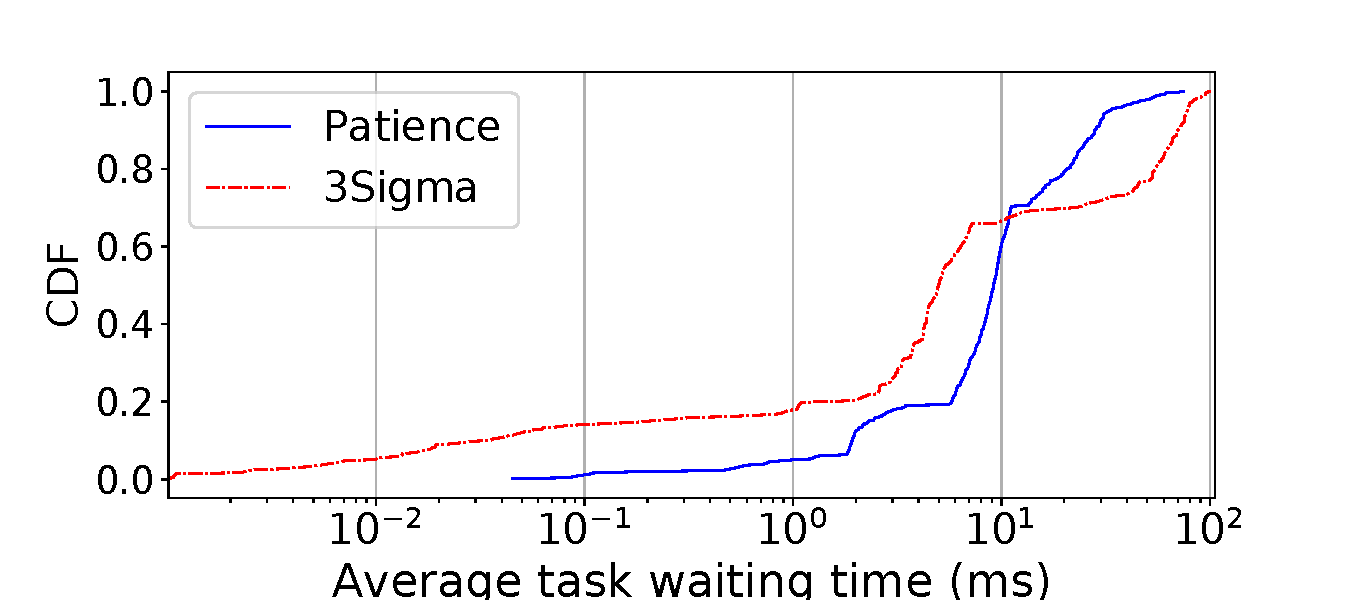
\includegraphics[width=0.9\linewidth]{figures/simulation/average_task_waiting_time_gTrace.pdf} %done
%	\label{fig:sim:waitingTimes:gTrace}
%	\vspace{-0.1in}
%}
%\subfigure[2STrace]{
%	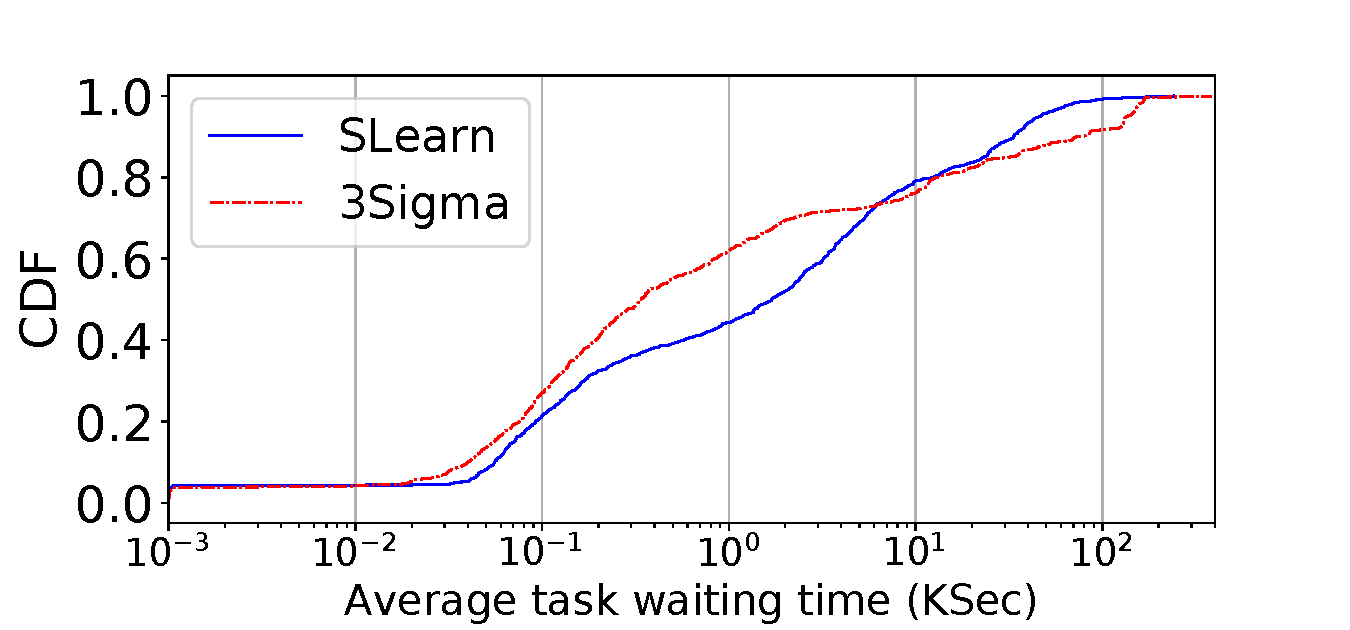
\includegraphics[width=0.9\linewidth]{figures/simulation/average_task_waiting_time_2STrace.pdf} %done
%	\label{fig:sim:waitingTimes:2Strace}
%	\vspace{-0.1in}
%}
%\caption{Waiting times for job.}
%\label{fig:intro:empAna}
%\vspace{-0.2in}
%\end{figure}

We summarize the major findings and contributions of this paper as follows:
\begin{itemize} %% [noitemsep,topsep=0pt,leftmargin=0.2in]
\item Based on literature survey and analysis using two different production
	cluster traces,
	%, one from Google and another 2Sigma, 
	we show that history is not a stable and accurate predictor for
	runtime characteristics of distributed jobs.

%\item We propose, \namepredict, the novel idea of applying sampling in the spatial dimension
\item We propose \lTechnique, a novel learning approach for distributed jobs.
\lTechnique uses sampling in the spatial dimension of jobs to learn job runtime
properties online with high accuracy.

\item Via quantitative, trace and experimental analysis, we demonstrate
  that \lTechnique can predict job runtime properties with much higher
  accuracy than history-based schemes. {For the 2Sigma~\cite{2Sigma:website},
 Google 2011~\cite{googleTraceGithub}, and
    Google 2019~\cite{, googleClusterData2019}
 cluster traces, the median prediction error are 18.98\%, 
13.68\%, and 51.84\% for \lTechnique but 36.57\%, 21.39\%, and 71.56\% for the
    state-of-the-art history-based \primarybasepredict.}
\item We show that learning job runtime properties by sampling
  job tasks, which conceptually delays scheduling the remaining tasks
  of a job, can be more than compensated by the improved accuracy, and
  as a result reduces the average JCT.
  In particular, our extensive simulations and testbed experiments
  using a prototype on a 150-node cluster
  in Microsoft Azure
  show that compared to the prior-art history-based predictor, \slearn
  reduces the average JCT by 1.28$\times$, 1.56$\times$, and 1.32$\times$ for the
  2Sigma, Google 2011 and Google 2019 traces, respectively.
\end{itemize}
